\documentclass[12pt]{article}
\usepackage[utf8]{inputenc}
\usepackage[draft]{moodle}
\usepackage{graphicx}

% Commands for jinja2 templating
% Instead of empty braces (i.e. no command effect), here we make the variable uppercase red
% to emphasize in the template those variables to be replaced. Once rendered, this formatting
% has not effect as jinja replaces the \VAR{variable} entirely.
\usepackage{xcolor}
\newcommand*{\VAR}[1]{\textcolor{red}{\textbf{#1}}}

%\moodle@draftmodetrue
%\moodle@draftmodefalse

\begin{document}
\begin{quiz}{Quiz No. \VAR{id}}
\begin{numerical}[points=2]{Basic addition}
What is \VAR{A} + \VAR{B}?
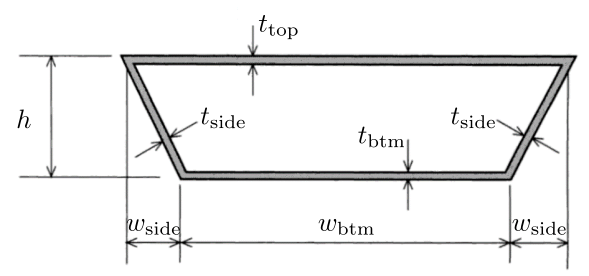
\includegraphics[width=8cm]{./media/image1}
\item \VAR{C}
\end{numerical}


\begin{shortanswer}[case sensitive=true]{Newton’s name}
What was Newton's first name?
\item* \VAR{text}
\item[fraction=0, feedback={No, silly!}] Fig
\item[fraction=0] Sir
\end{shortanswer}
\begin{multi}[points=3]{A first derivative}
What is the first derivative of $x^3$?
\item $\frac{1}{4} x^4+C$
\item* $3x^2$
\item \VAR{D}
\end{multi}
\end{quiz}

\end{document}
